\section{Cell Error}
Once the Voronoi tessellation is determined, it is re-centred based on the weighted average of the points in the cell. Sources are added to cells by determining the cell centre which is closest to it using the standard distance equation:
\begin{equation}
d = \sqrt{(x_i - x_c)^2 + (y_i - y_c)^2},
\end{equation}
where $(x_i,y_i)$ is the location of a source in the plane and $(x_c,y_c)$ is the location of a centre. The closest centre is such that $d$ is minimum. This is done to add the influence of weaker sources in overall correction. This is especially necessary when the cell is generated by a source slightly above the intensity threshold and contains a source slightly below the threshold. We seek a new weighted centre such that the error for a cell is minimum. The error for a cell containing $N$ sources is defined as
\begin{equation} \label{eq:cellerr}
	\epsilon = \sum^N_{i=0} z_i|\vec{r_i} - \vec{r_c}|^2,
\end{equation}
with $\vec{r_i} = (x_i,y_i)$ is the location and $z_i$ is the intensity of some source in the cell and $\vec{r_c}$ as the location of a new centre. 
\\
This error function will have a local minima at the point where its derivative with regards to $\vec{r_c}$ is zero, or
\begin{align*}
	\frac{d\epsilon}{d\vec{r_c}} &= \sum^N_{i=0} \frac{d}{d\vec{r_c}}z_i(|\vec{r_i}|^2 -2\vec{r_i}\cdot\vec{r_c} + |\vec{r_c}|^2) \\
	&= \sum^N_{i=0} z_i(2\vec{r_i} - 2\vec{r_c}) = 0 \\
\end{align*}
or
\begin{equation*}
	2\sum^N_{i=0} z_i\vec{r_i} = 2\sum^N_{i=0}z_i\vec{r_c}
\end{equation*}
Since $\vec{r_c}$ is not dependant on the sum, it can be removed and the equation reordered to give
\begin{equation}
	\vec{r_c} = \frac{\sum^N_{i=0} z_i\vec{r_i}}{\sum^N_{i=0}z_i}
\end{equation}
From this, the new centre is determined, since it is required for the cell merge, the new centre retains the old centres intensity value i.e. the highest intensity from a source in the cell. Once the cell's new centre is obtained, its error is calculated using Equation \ref{eq:cellerr}. An example of centre correction can be seen in the difference between Figure \ref{fig:recen1} and Figure \ref{fig:recen2}.
\begin{figure}[H]
  \centering
  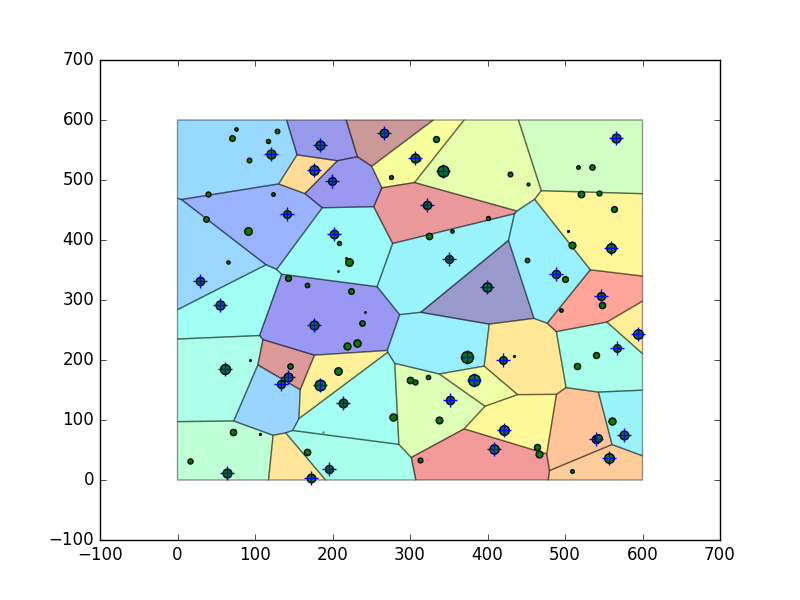
\includegraphics[width=0.8\textwidth]{Images/recentre1.png}
  \caption{Tessellation with high intensity points as centres.}
  \label{fig:recen1}
\end{figure}
\begin{figure}[H]
  \centering
  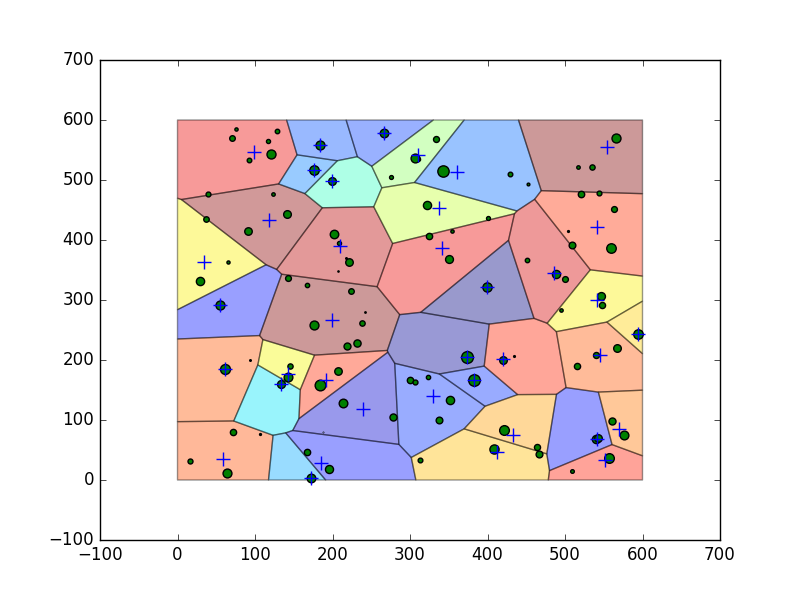
\includegraphics[width=0.8\textwidth]{Images/recentre2.png}
  \caption{Tessellation with the weighted average of the points in the cells as their centres.}
  \label{fig:recen2}
\end{figure}